% Gemini theme
% https://github.com/anishathalye/gemini

\documentclass[final]{beamer}

% ====================
% Packages
% ====================

\usepackage[T1]{fontenc}
\usepackage{lmodern}
\usepackage[size=custom,width=120,height=72,scale=1.0]{beamerposter}
\usetheme{gemini}
\usecolortheme{gemini}
\usepackage{graphicx}
\usepackage{booktabs}
\usepackage{tikz}
\usepackage{pgfplots}
\pgfplotsset{compat=1.14}
\usepackage{anyfontsize}
\usepackage{amsmath}
\usepackage{algorithmic}
\usepackage{bm}
\usepackage{listings}
\usepackage[font={scriptsize,it}]{caption}

% ====================
% Lengths
% ====================

% If you have N columns, choose \sepwidth and \colwidth such that
% (N+1)*\sepwidth + N*\colwidth = \paperwidth
\newlength{\sepwidth}
\newlength{\colwidth}
\setlength{\sepwidth}{0.025\paperwidth}
\setlength{\colwidth}{0.3\paperwidth}

\newcommand{\separatorcolumn}{\begin{column}{\sepwidth}\end{column}}

% ====================
% Title
% ====================

\title{PCquery.jl: Automated Mining, Integration, and Annotation of Biological Signaling Pathways}

\author{Matthew Karikomi \inst{1,2,3} \and Qing Nie \inst{2,3}}

\institute[shortinst]{\inst{1} Mathematical, Computational, and Systems Biology Program \samelineand \inst{2} Department of Mathematics, UC Irvine \samelineand \inst{3} NSF-Simons Center for Multiscale Cell Fate Research}

% ====================
% Footer (optional)
% ====================

\footercontent{
  \href{https://github.com/mkarikom/PCquery.jl}{https://github.com/mkarikom/PCquery.jl} \hfill
  SoCal SysBio 2023, Los Angeles \hfill
  \href{mailto:mkarikom@uci.edu}{mkarikom@uci.edu}}
% (can be left out to remove footer)

% ====================
% Logo (optional)
% ====================

% use this to include logos on the left and/or right side of the header:
% \logoright{\includegraphics[height=7cm]{logo1.pdf}}
% \logoleft{\includegraphics[height=7cm]{logo2.pdf}}

% ====================
% Body
% ====================

\begin{document}

\addtobeamertemplate{headline}{}
{	
	\begin{tikzpicture}[remember picture,overlay]
	\node [anchor=north west, inner sep=3cm] at ([xshift=-0.5cm,yshift=2.2cm]current page.north west)     {
\includegraphics[height=7cm]{Image/UCI_SEAL}};
	\end{tikzpicture}
	
	\begin{tikzpicture}[remember picture,overlay]
	\node [anchor=north east, inner sep=3cm] at ([xshift=0cm,yshift=1.2cm]current page.north east)     {
\includegraphics[height=5.5cm]{Image/cmcf}};
	\end{tikzpicture}
}

\begin{frame}[t,fragile]
\begin{columns}[t]
\separatorcolumn

\begin{column}{\colwidth}  
  \begin{exampleblock}{BioPAX is a graph-based representation of knowledge}
    Pathways in BioPAX \cite{demir2010biopax} are heterogeneous graphs whose edges denote both conceptual (relational) knowledge and dynamics.
    \begin{figure}
      \centering
      \begin{minipage}{0.4\textwidth}
        \footnotesize
        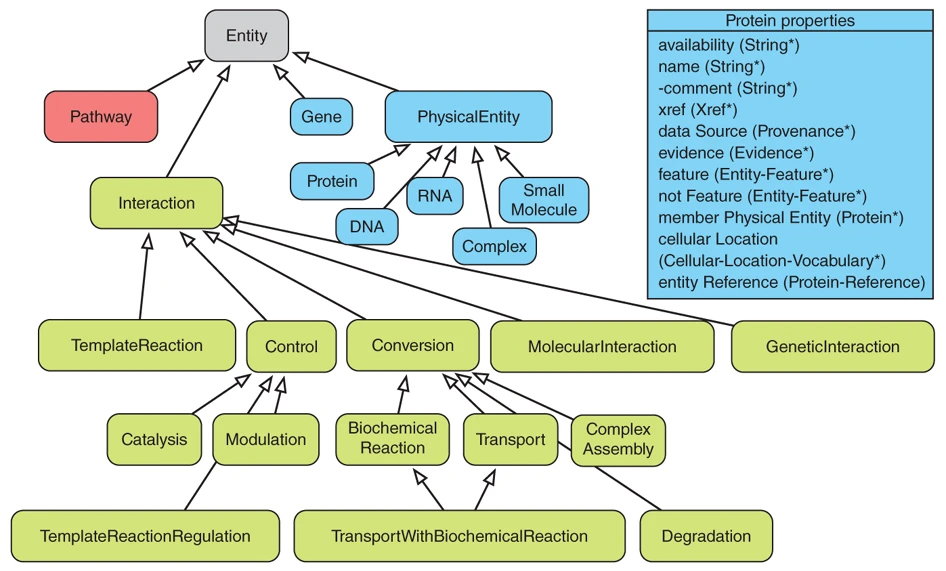
\includegraphics[scale=0.45]{Image/biopax_schema.jpg}
        \caption{BioPAX knowledge schema.  Image credit: \cite{demir2010biopax}}
      \end{minipage}
      \hspace{2.5cm}
      \begin{minipage}{0.4\textwidth}
        \footnotesize
        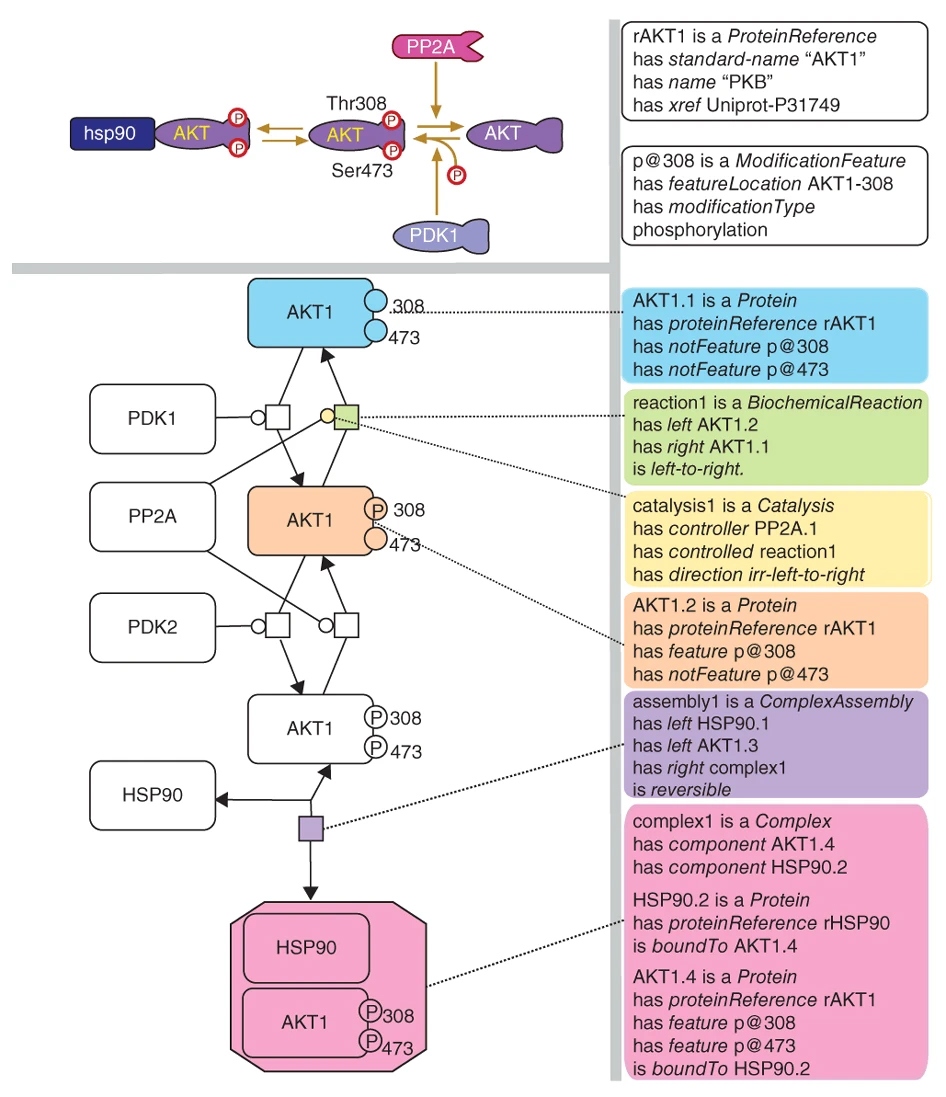
\includegraphics[scale=0.35]{Image/biopax_akt.jpg}
        \caption{Representation of a unique macromolecular state in BioPAX.  Image credit: \cite{demir2010biopax}}
      \end{minipage}
    \end{figure}
  \end{exampleblock}

  \begin{block}{Pathways can be mined programmatically}
    Curated pathway databases, such as Reactome \cite{fabregat2018reactome} and KEGG \cite{kanehisa2007kegg}, are aggregated by the PathwayCommons \cite{rodchenkov2020pathway} initiative and ported to BioPAX, allowing PCquery to mine sets of related pathways using structured queries:
    \footnotesize
    \begin{lstlisting}
      psParams = Dict(
        "q"=>"notch1",:filter=>[["notch1","nucleus"],["notch1","transcription"]],
        "type"=>"pathway","datasource"=>"reactome")
    \end{lstlisting}

    \begin{figure}
      \centering
      \footnotesize
      \begin{minipage}{0.45\textwidth}
        \includegraphics[scale=3.0]{Image/notch1membrane.pdf}
        \caption{Notch1 Cytosolic Pathway\newline(Reactome HSA-2122948)}
      \end{minipage}
      \hspace{2.5cm}
      \begin{minipage}{0.45\textwidth}
        \includegraphics[scale=3.0]{Image/notch1nucleus.pdf}
        \caption{Notch1 Nuclear Pathway\newline(Reactome HSA-2122947)}
      \end{minipage}
    \end{figure}
  \end{block}

  \begin{exampleblock}{Enumerate nested surface-marker interactions}
    \begin{figure}
      \centering
      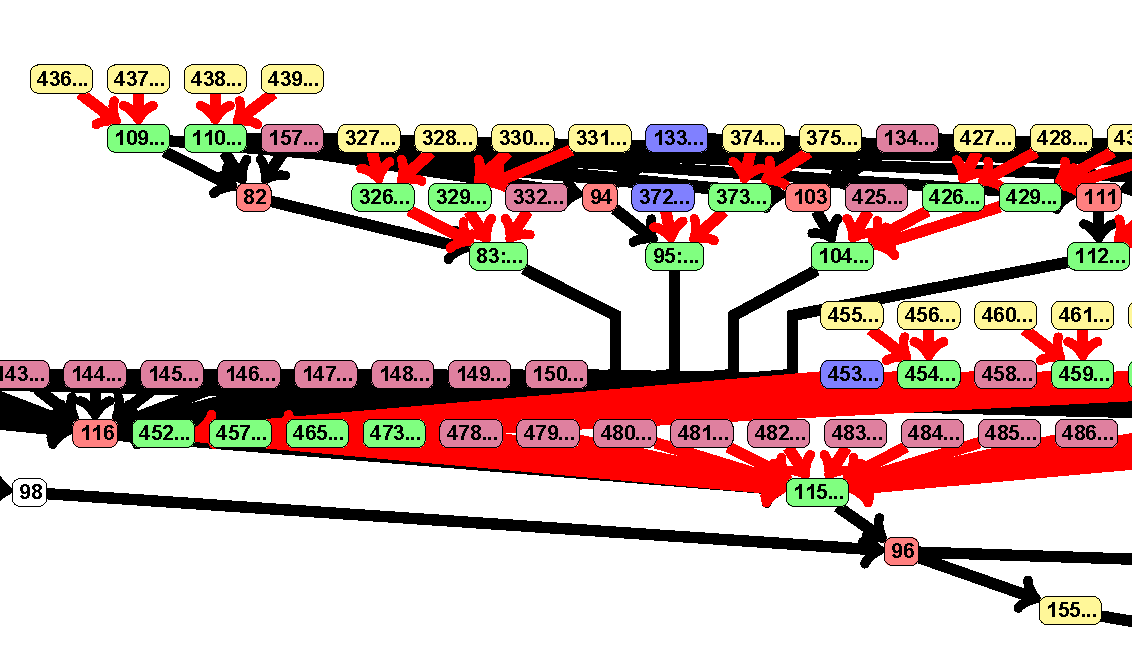
\includegraphics[scale=1.0]{Image/ontology_enumeration_NODEID.pdf}
      \caption{Expansion of complexes imputes complex-forming interactions and allows GO annotation of reactants to be mined from NextProt \cite{lane2012nextprot}}
    \end{figure}
  \end{exampleblock}

\end{column}

\separatorcolumn

\begin{column}{2\colwidth}
  \begin{block}{Multi-pathway scope}
    Model-selection tasks requiring marker IDs from multiple contexts (e.g. cytosolic, nuclear) can be executed within the context of the integrated graph, as shown below for ligand-receptor interactions in the Notch pathway, including the transcriptional targets of Jag1.
    
    \begin{figure}
      \centering
      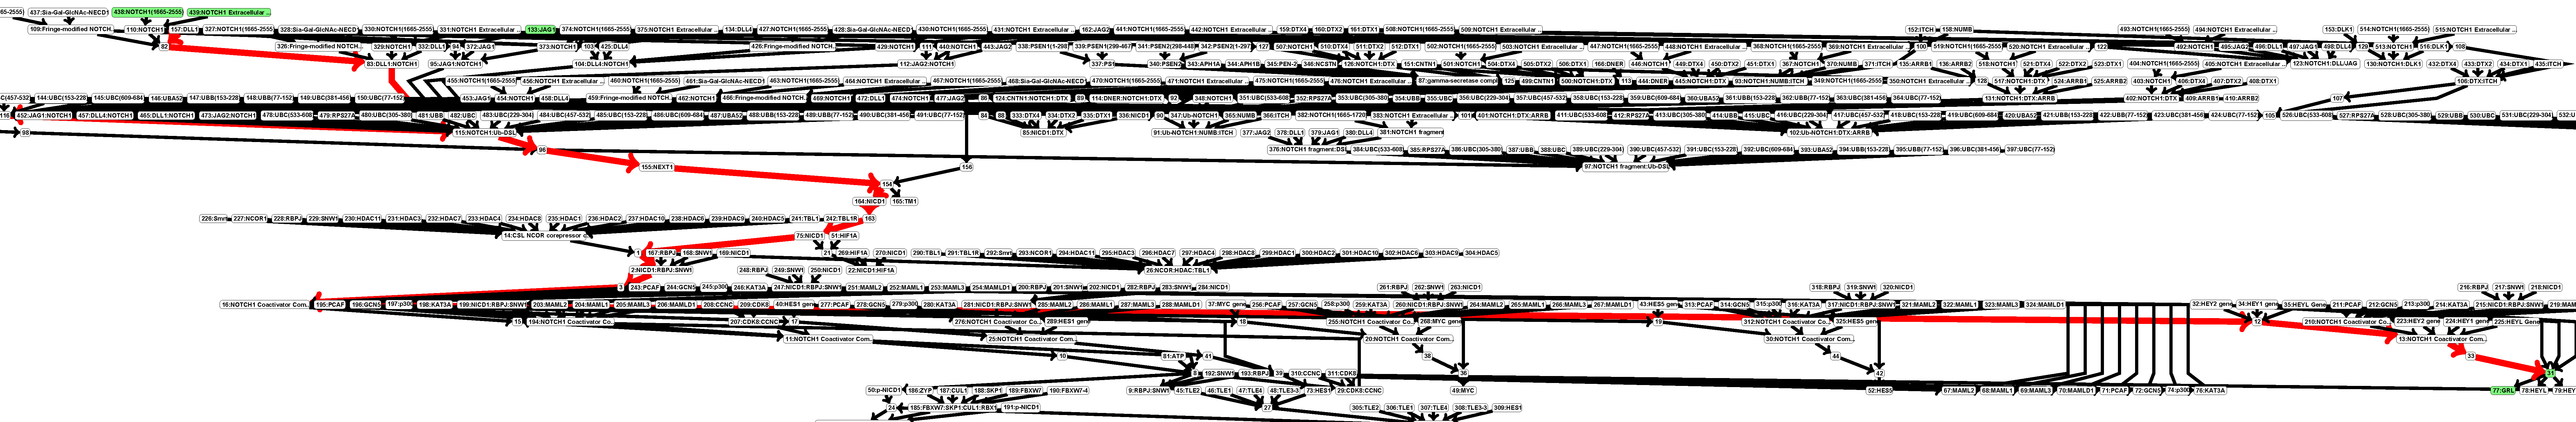
\includegraphics[scale=0.5]{Image/notch_path.pdf}
      \caption{Integrated signaling graph for human Notch1.}
    \end{figure}
    
  \end{block}
  \begin{columns}[t] % Split up the two columns wide column again
    \begin{column}{1.3\colwidth}
      \begin{block}{Package Workflow}

        Workflow begins with keyword-based search of knowledge graphs from the PathwayCommons \cite{rodchenkov2020pathway} online database, which aggregates annotated pathways in BioPAX \cite{demir2010biopax}.  Individual pathways are integrated via common molecular identifiers.   Once this integrated graph is constructed, PCquery traverses the graph and further labels all vertices with annotations from other online databases, including gene, transcript, and GO terms from NextProt \cite{lane2012nextprot}, and inter-species gene and transcript orthologs from OrthoDB \cite{kriventseva2019orthodb}.
        
        \begin{figure}
          \centering
          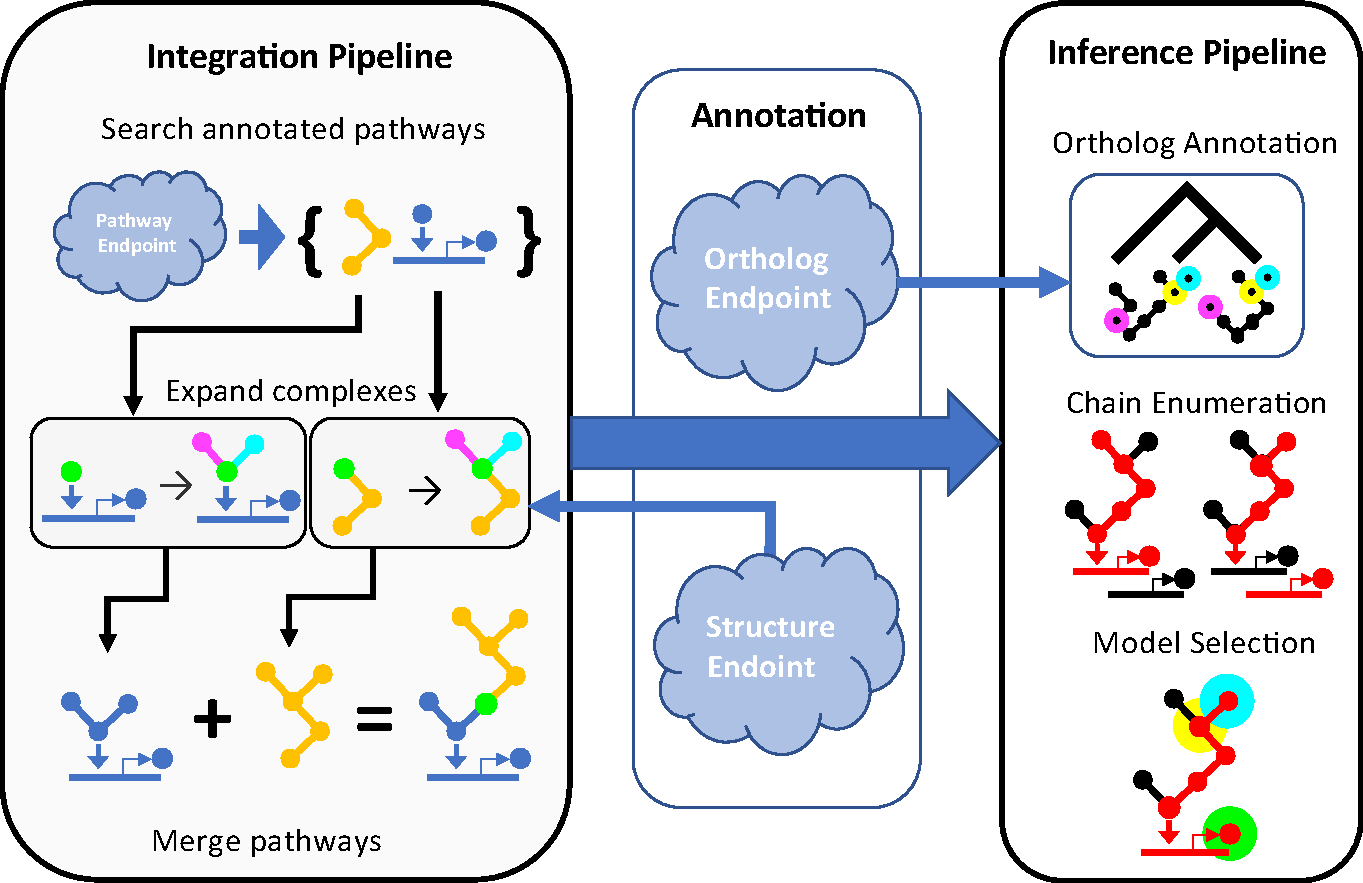
\includegraphics[scale=1.5]{Image/schematic.pdf}
          \caption{A) query BioPAX pathway repository based on organism and keyword search.  B) for each annotated pathway (blue,yellow) recursively impute complex-forming reactions (RHS blue arrow) based on existing product annotations (green) and their BioPAX-annotated constituents (purple,blue).  C) Integrate augmented pathways (blue, yellow) based  on common molecular identifiers (green).  D) Mine inter-species pathway markers based on sequence-homology between reference integrated pathway protein gene loci and the gene loci of the target species.  E) Enumerate signaling trajectories for integrated pathways.  Query gene regulatory interactions downstream of cell-surface interactions based on GO annotation of integrated pathways.}
        \end{figure}

      \end{block}
    \end{column}
    \begin{column}{0.7\colwidth}
    
      \begin{exampleblock}{Interspecies ortholog expression}
    
        \begin{figure}
          \centering
          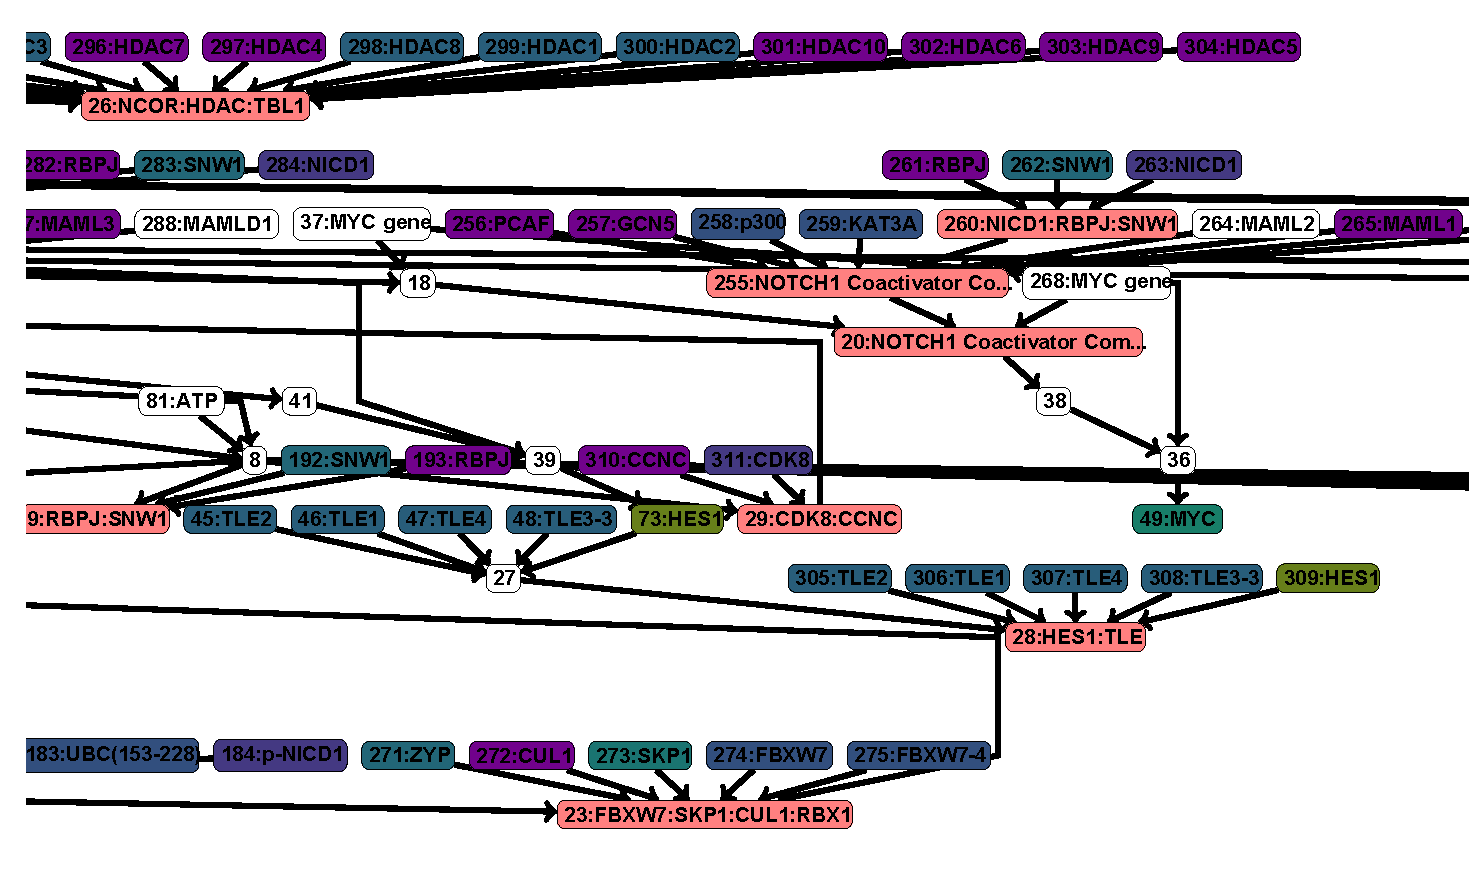
\includegraphics[scale=0.75]{Image/orthomap_GID.pdf}
          \caption{Mapping the gene expression of a single zebrafish neural crest cell to human orthologs in the integrated Notch1 pathway from human}
        \end{figure}
    
      \end{exampleblock}
      \begin{block}{References}
        \nocite{*}
        \tiny{\bibliographystyle{plain}\bibliography{poster}}      
      \end{block}
  \end{column}
\end{columns}
  

\end{column}

\separatorcolumn
\end{columns}
\end{frame}

\end{document}
